\documentclass{article} % For LaTeX2e
\usepackage{nips15submit_e,times}
\usepackage{hyperref}
\usepackage{url}
\usepackage{graphicx}
%\documentstyle[nips14submit_09,times,art10]{article} % For LaTeX 2.09



\begin{document}

\section{Models}
\subsection{Convolution Neural Network}
Our CNN model consists of eleven layers: two 2D convolution layers followed by a max pooling layer, then three alternating 2D convolution layers and max pooling layer pairs, then two dense layers at the end. In each layer, we used rectified linear units as the activation (ReLU), with the exception of the final categorisation layer, for which we used a softmax activation. 
 
\subsection{Recurrent Neural Network}

We implemented an RNN-based version of the above, which first performs 2D convolutions reducing the size of the spectrogram in the frequency domain. Then, an LSTM is used to iterate through the time domain. The final layer of this LSTM is fed to a fully connected layer reducing this to 11 nodes; the output of these are input to a softmax function yielding a probability distribution over the categories.

The architecture of the convolution component which preceeds the LSTM is:

\begin{enumerate}
\item 2x2 convolution
\item 2x2 convolution
\item 2x4 max-pooling
\item five of
\begin{enumerate}
\item 2x2 convolution
\item 2x1 max pooling
\end{enumerate}
\end{enumerate}

at which point the frequency domain has been reduced by a factor of approximately $2^6$ and the time domain by a factor of 4.

\section{Results}
\subsection{Convolution Neural Network}
We split our data into training and test sets, using six speakers for training (three male, three female) and four speakers for the test set (two male, two female). This lead to 132 samples in the training set and 88 samples in the test set. We trained the CNN using a batch size of four. For our loss function, we minimised the categorical-crossentropy.

We began by using the state-of-the-art adadelta optimiser, for training for twelve epochs. For our first runs, we did not augment the data set. We ran the network six times and obtained a wide range of results for the test accuracy. Five of the six results were in the range 0.8750-0.9432, the other was 0.0909 which, with eleven categories, is equivalent to random guessing. The validation and test accuracy for one run, as the number of epochs increases, is shown in Figure \ref{fig:2d_acc}. It appears that we are overfitting to the training data, given that the validation accuracy goes to 1. 

\begin{figure}[h]
\begin{center}
%\framebox[4.0in]{$\;$}
%\fbox{\rule[-.5cm]{0cm}{4cm} 
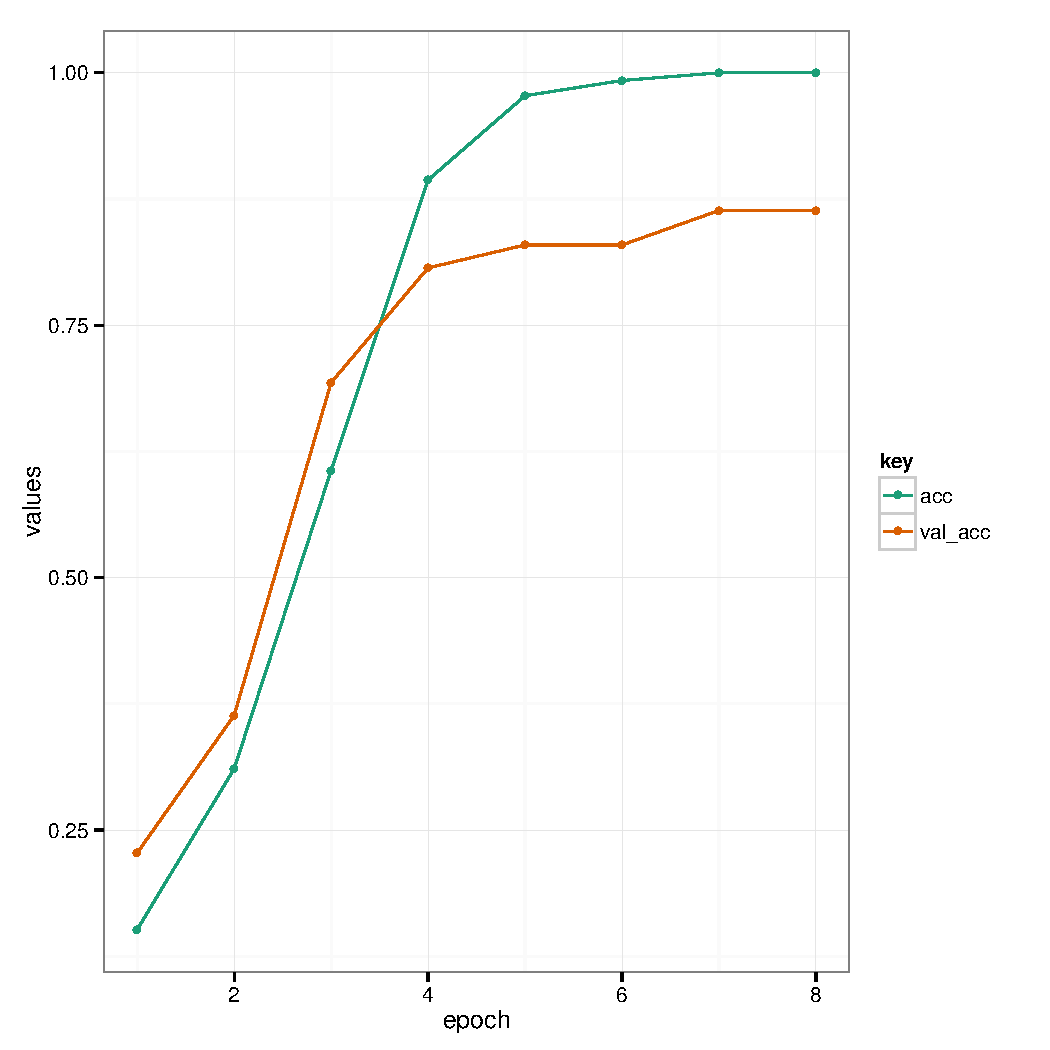
\includegraphics[height = 4in, width = 4in]{cnn_2d_plot_acc.pdf}
%\rule[-.5cm]{4cm}{0cm}}
\end{center}
\caption{Validation (red) and test (green) accuracy for the CNN on one run, with unaugmented data.}
\label{fig:2d_acc}
\end{figure}

We then ran the model with leave-one-out cross-validation (LOOCV), training on nine of the speakers and testing on the tenth. Three times out of 10, the test accuracy was 1, twice it was 0.8636 and the other half of the times it was just 0.0909.

We experimented with adding dropout layers to the CNN in an attempt to address overfitting, but did not see any improvements in the test accuracy as a result. In an attempt to improve performance, we augmented the data by copying and shifting the signal of the audio files of the training data before computing the mfsc. We shifted each training sample by each of two, four, six, eight and ten 8000th of a second to both the left and right, resulting in eleven very slightly varying training samples for every one in the original runs. This increase in the training set meant that fewer epochs were required for convergence, with results stabilising after around five. When using the original training/test data split, it also lead to some higher test score accuracy than in the un-augmented case, though there was still a range of results, from 0.8750-0.9659, with occasional results of 0.0909. It is not clear whether the augmentation of the data led to an improved classifier or whether the higher scores are down to some of the randomness inherent in the process.
LOOCV on the augmented training set faced similar issues as on the original set; whilst five scored highly, the other five were essentially guesses.

We also explored augmenting the original dataset by adding some white noise to the background of the audio signal, but this did not make any appreciable difference to the test scores, likely because the original audio files were all recorded in controlled settings, so there was no noise in the test set.

Since our classifer was on occasion producing very high losses, we explored the possibility that this might be because the learning rate was too high, and so ran our model again with the but optimising with stochastic gradient descent (SGD), rather than adadelta, and running for 20 rather 12 epochs. Applying LOOCV on the un-augmented training set resulted in a test accuracy of 0.8636. As with LOOCV using adadelta, the test accuracy varied greatly in each fold, ranging from 0.4545 to 1, though unlike the previous case, even its worse performance was a significant improvement on random guessing. An area of further research would be to experiment with the tuning parameters of SGD (learning rate, momentum and decay) to see if we can reduce the range and improve the average test accuracy. It would also be interesting to examine the audio files and mfsc representation of the test samples in the folds where the test accuracy was low to determine whether there is anything in particular about those speakers which makes their spoken digits harder to classify. 


\end{document}
